\chapter{神经网络的基础知识}

\section{神经网络的运行原理} \label{nn-principal}

本节中将以最基本的全连接前馈神经网络为例,介绍神经网络的基本运行原理。

训练神经网络是以让神经网络拟合任意的函数为目标的。例如,在图像分类任务中,神经网络输入的是从图片中提取的特征,输出的是该图片是每一分类的得分。训练的目标就是让神经网络输出中正确的一类的得分尽可能高。

神经网络模型的开发过程一般是,搭建模型的结构,然后反复运行前向传播,反向传播,优化这三个步骤,直至收敛。

\subsection{前向传播} \label{nn-forward}

\begin{figure}[]
    \centering
    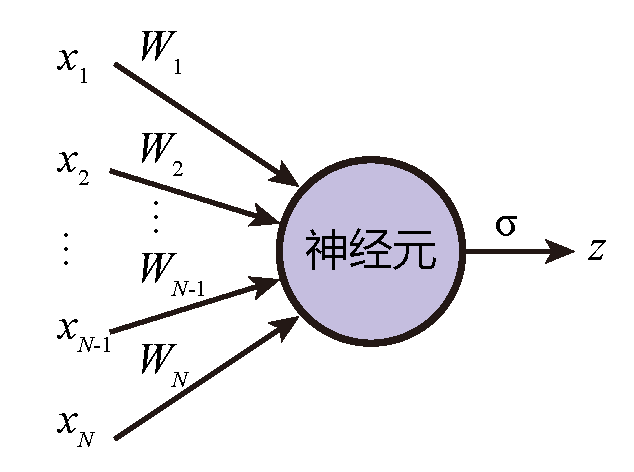
\includegraphics[page=1]{figure/figures.pdf}
    \caption{神经元示意图}
    \label{nunit}
\end{figure}

如图\ref{nunit}所示,神经元是全连接前馈神经网络的基本单元。每个神经元接收若干个信号输入,经过与神经元的权重连接(线性变换)和激活函数(非线性变换)之后,输出一个新的信号。具体来说,神经元接受一个N维向量$\bm{x}\in\mathbb{R}^N$作为输入,则其输出为:
\begin{equation}
    z=\sigma\left(\bm{W}\bm{x}+b\right)
\end{equation}

其中$\bm{W}\in\mathbb{R}^N$是该神经元连接的权重,是可学习的参数。$b$是可选的偏置项,也是可学习的参数,$\sigma$是非线性激活函数。

$M$个接受相同输入的神经元构成了一层神经网络,每个神经元具有不同的可学习参数。则一层神经网络的运行也可以表示为:
\begin{equation}
    \bm{z}=\sigma\left(\bm{W}\bm{x}+\bm{b}\right)
\end{equation}

其中$\bm{W}\in\mathbb{R}^{M\times N}$是该层所有神经元的连接的权重,$\bm{b}\in\mathbb{R}^M$是该层所有神经元的偏置项。$\bm{z}\in\mathbb{R}^M$是该层所有神经元的输出,它可能是模型最后的输出,也可能是下一层神经元的输入。

\begin{figure}[]
    \centering
    \includegraphics[page=2]{figure/figures.pdf}
    \caption{神经网络示意图}
    \label{nnet}
\end{figure}

通常神经网络会由至少三层神经元构成。如图\ref{nnet}所示,第一层称为输入层,其输入是原始的特征向量,最后一层称为输出层,其输出为模型最终的输出,其余的则称为隐藏层,将上一层的输出作为输入,自己的输出则作为下一层的输入。每一层的神经元的数量可以不同。但上一层的神经元数量应和下一层的输入向量的长度是一致的。对于有L层的神经网络来说,若$\bm{x}^0$为表示原始特征的向量,则第l层的输出可以表示为:
\begin{equation}
    \bm{x}^l=\sigma\left(\bm{W}^l\bm{x}^{l-1}+\bm{b}^l\right),l\in\left\{1,2,\ldots,L\right\}
\end{equation}

$\bm{x}^L$即为网络最终的输出。

\begin{figure}[]
    \centering
    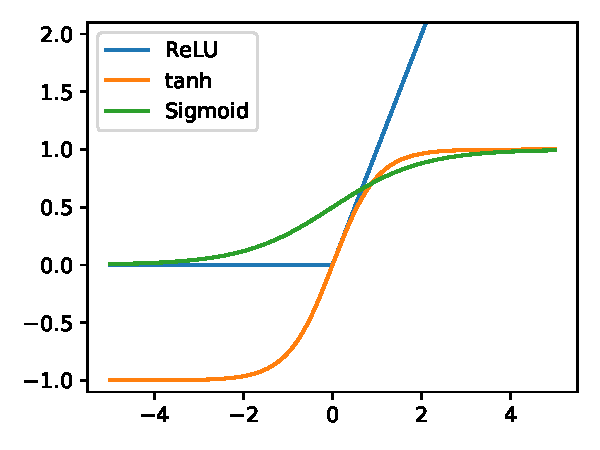
\includegraphics{figure/act.pdf}
    \caption{激活函数}
    \label{act-func}
\end{figure}

对于激活函数,理论上它可以是任何连续的非线性函数。若没有激活函数,则整个网络将只有线性变换,无论使用多复杂的结构,输出也只能是输入向量的线性变换,其表达能力十分有限。常用的激活函数有ReLU,tanh,sigmoid等。如图\ref{act-func}所示,以下是它们的定义:
\begin{align}
    \mathrm{ReLU}\left(x\right)&=\max{\left(x,0\right)}\\
    \tanh{\left(x\right)}&=\frac{e^x-e^{-x}}{e^x+e^{-x}}\\
    \mathrm{sigmoid}\left(x\right)&=\frac{1}{1+e^{-x}}
\end{align}

以上介绍的从$\bm{x}^0$计算得到$\bm{x}^L$的过程即为模型的前向传播过程。在前述图像分类任务中,$\bm{x}^L$中即包含了预测的图像属于每一分类的得分。在实际更复杂的神经网络中,在前向传播的过程中可使用任何连续可导的运算,并不局限于上述提到的表达式。

\subsection{反向传播}

反向传播的目的是为网络中的每一个可学习的参数计算一个梯度,当将这些参数的数值向梯度的相反方向移动的时候,我们期望模型在下一次迭代的时候可以做得更好,得出更加正确的结果。为了得到这样的梯度,我们需要一个函数,对模型的输出进行评价,其函数值越小,则代表模型在该任务上的表现越好。这样的函数称作损失函数 (loss function)。我们所期望求得的梯度就是损失函数的梯度了。根据任务的不同,我们会设计不同的损失函数。以之前提到的图片分类任务为例,最常用的损失函数为交叉熵 (cross entropy) 损失函数,其针对单个输入样本的定义为:
\begin{equation}
    \mathrm{CE}\left(\bm{x},y\right)=-\log{\left(\frac{\exp{\left(\bm{x}_y\right)}}{\sum_{j=1}^{N}\exp{\left(\bm{x}_j\right)}}\right)}
\end{equation}

其中$N$为分类的数量,$\bm{x}\in\mathbb{R}^N$为模型输出的各个分类的得分,$y$为正确的分类的下标。正确的分类的得分越高,其他分类的得分越低,该函数的函数值就越小,越趋近于0。
下面以\ref{nn-forward}节介绍的全连接前馈神经网络中的参数$\bm{W}^l$为例,介绍反向传播的计算过程。其基本思路是函数的链式求导法则。具体来说,我们所要求的梯度是:
\begin{equation}
    \nabla\bm{W}^l=\frac{\partial J\left(\cdot\right)}{\partial\bm{W}^l}
\end{equation}

其中$J\left(\cdot\right)$为损失函数。

在反向传播的过程中,我们从输出层至输入层,反向逐层求解每层的梯度。损失函数的导数将根据损失函数的不同而不同,为讨论方便,我们假设损失函数的偏导数$\frac{\partial J\left(\cdot\right)}{\partial\bm{x}^L}$为已知的。同样地,我们假设激活函数$\sigma$的导数是已知的。一般地,对于第$l$层神经网络,令:
\begin{equation}
    \bm{z}^l=\bm{W}^l\bm{x}^{l-1}+\bm{b}^l
\end{equation}

则:
\begin{align}
    \frac{\partial J\left(\cdot\right)}{\partial\bm{z}^l}&=\frac{\partial\bm{x}^l}{\partial\bm{z}^l}\cdot\frac{\partial J\left(\cdot\right)}{\partial\bm{x}^l}\\
    &=\frac{\partial J\left(\cdot\right)}{\partial\bm{x}^l}\odot\sigma^\prime\left(\bm{z}^l\right)\\
\
    \frac{\partial J\left(\cdot\right)}{\partial\bm{W}^l}&=\left[\frac{\partial J\left(\cdot\right)}{\partial\bm{W}_{ij}^l}\right]_{ij}\\
    &=\left[\frac{\partial\bm{z}_i^l}{\partial\bm{W}_{ij}^l}\cdot\frac{\partial J\left(\cdot\right)}{\partial\bm{z}_i^l}\right]_{ij}\\
    &=\left[\bm{x}_j^{l-1}\cdot\frac{\partial J\left(\cdot\right)}{\partial\bm{z}_i^l}\right]_{ij}\\
    &=\frac{\partial J\left(\cdot\right)}{\partial\bm{z}^l}\cdot\left(\bm{x}^{l-1}\right)^T\\
\
    \frac{\partial J\left(\cdot\right)}{\partial\bm{x}^{l-1}}&=\frac{\partial\bm{z}^l}{\partial\bm{x}^{l-1}}\cdot\frac{\partial J\left(\cdot\right)}{\partial\bm{z}^l}\\
    &=\left(\bm{W}^l\right)^T\cdot\frac{\partial J\left(\cdot\right)}{\partial\bm{z}^l}
\end{align}

其中,$\odot$表示逐元素相乘。$\delta^l=\frac{\partial J\left(\cdot\right)}{\partial\bm{z}^l}$也被称为残差。利用上述公式,我们即可从最后一层开始,计算出每一个$\nabla\bm{W}^l$。

\subsection{梯度下降优化}

当我们为每一个参数在反向传播中计算了梯度之后,需要使用优化算法利用求得的梯度将模型更新到更好的算法。以下以最简单的随机梯度下降 (stochastic gradient descent) 方法为例,并以$\theta^i$表示第i次迭代时模型的所有参数,以$\nabla\theta^i$表示它们的梯度:
\begin{equation}
    \theta^{i+1}=\theta^i-\alpha\cdot\nabla\theta^i
\end{equation}

其中$\alpha$表示学习率,是可以调整的超参数。除了简单的随机梯度下降方法外,还有一些著名的优化算法,如带有动量的随机梯度下降 (stochastic gradient descent with momentum),Adam\cite{Adam14}等。

在实际过程中,从单个训练样例中计算得到的梯度将难以反应整个数据集上的数据分布情况,而如果每次迭代都使用整个数据集的样例计算平均梯度则显得浪费计算资源。所以我们一般在每次迭代时从训练集中选出一小批样例并计算它们的平均梯度,称作小批量梯度下降 (mini-batch gradient descent) 方法。

\section{循环神经网络 (RNN)}

\ref{nn-principal}节中描述的全连接前馈神经网络只能处理固定长度的特征。这对于例如图片等数据是没有问题的,图片总是能采样到任何希望的大小。然而对于例如自然语言的输入来说,每次输入的长度都是不一样的,神经网络需要有一种机制来处理变长的输入。循环神经网络就应运而生了。

循环神经网络的输入$\bm{X}=\left\{\bm{x}_1,\bm{x}_2,\ldots,\bm{x}_N\right\}$为长度为$N$的序列,序列中每个元素为一个表示该元素特征的向量,其输出$\bm{Y}=\left\{\bm{y}_1,\bm{y}_2,\ldots,\bm{y}_N\right\}$也是长度为$N$的序列。$N$可以随时改变。以自然语言的文本数据为例,语句中的每个单词可以作为输入序列中的一个元素,其向量表示可以来自预先训练的表示,也可以随机初始化词嵌入向量,并将其随模型一起训练。

\subsection{Vanilla RNN}

\begin{figure}[]
    \centering
    \includegraphics[page=3]{figure/figures.pdf}
    \caption{Vanilla RNN单元}
    \label{vanilla-rnn}
\end{figure}

如图\ref{vanilla-rnn}所示,Vanilla RNN 的前向传播过程与\ref{nn-principal}节中描述的全连接前馈神经网络有相似之处,它的前向传播算法如下:
\begin{align}
    \bm{h}_t&=\sigma\left(\bm{W}_{hx}\bm{x}_t+\bm{W}_{hh}\bm{h}_{t-1}+\bm{b}_h\right)\\
    \bm{y}_t&=\bm{W}_{yh}\bm{h}_t+\bm{b}_y
\end{align}

其中$\bm{W}_{hx}\in\mathbb{R}^{h\times x},\bm{W}_{hh}\in\mathbb{R}^{h\times h},\bm{W}_{yh}\in\mathbb{R}^{y\times h},\bm{b}_h\in\mathbb{R}^h,\bm{b}_y\in\mathbb{R}^y$均为可学习的参数,$\bm{h}_t$为第$t$次迭代时的隐藏层状态,$\sigma$为激活函数。它和全连接网络一样,都是由线性变换和激活函数组成。不同的是,RNN在每次迭代中使用相同的权重,这就是它称为“循环”的原因,并且它在每次迭代时还接受新的输入$\bm{x}_t$,这样只需调整迭代的次数就能处理不同长度的输入了。此外,由于网络按顺序接受每个输入,它还能捕获到输入中的时序信息,例如自然语言中每个词语的前后顺序,这样的信息在实际中是非常重要的。

但Vanilla RNN具有梯度消失或爆炸的问题,这会严重阻碍模型学习到合适的权重,特别是难以建模长时间间隔状态之间的依赖关系,因此在实际中并不是很常用。

\subsection{LSTM}

\begin{figure}[]
    \centering
    \includegraphics[page=4,width=\linewidth]{figure/figures.pdf}
    \caption{LSTM单元}
    \label{lstm}
\end{figure}

如图\ref{lstm}所示,长短时记忆 (long short-term memory, LSTM)\cite{lstm97}网络是一种当前使用广泛的RNN网络。LSTM除了拥有Vanilla RNN的处理变长输入,捕获时序关系的优点,还中引入了门控机制来控制信息的累计速度,包括有选择地加入新的信息,并有选择地遗忘之前累计的信息,以此来建模长期的依赖关系。LSTM的前向传播过程较为复杂,如下所示:
\begin{align}
\bm{i}_t&=\sigma\left(\bm{W}_i\ \bm{x}_t+\bm{U}_i\ \bm{h}_{t-1}+\bm{b}_i\right)\\
\bm{f}_t&=\sigma\left(\bm{W}_f\bm{x}_t+\bm{U}_f\bm{h}_{t-1}+\bm{b}_f\right)\\
\bm{o}_t&=\sigma\left(\bm{W}_o\bm{x}_t+\bm{U}_o\bm{h}_{t-1}+\bm{b}_o\right)\\
{\widetilde{\bm{c}}}_t&=\tanh{\left(\bm{W}_c\bm{x}_t+\bm{U}_c\bm{h}_{t-1}+\bm{b}_c\right)}\\
\bm{c}_t&=\bm{f}_t\odot\bm{c}_{t-1}+\bm{i}_t\odot{\widetilde{\bm{c}}}_t\\
\bm{h}_t&=\bm{o}_t\odot\tanh{\left(\bm{c}_t\right)}
\end{align}

其中$\bm{W},\bm{U},\bm{b}$均为可学习的参数,$\sigma$为sigmoid函数。$\bm{i}$为输入门,$\bm{f}$为遗忘门,$\bm{o}$为输出门,$\bm{c}$为记忆单元,$\bm{h}$为输出的隐藏状态。LSTM在记忆单元中保存需要长期保存的信息,并通过输入门控制有多少新的信息进入记忆单元,通过遗忘门控制有多少旧的信息要保留在记忆单元中,并通过输出门控制当前隐藏状态的输出信息。通过广泛使用门控机制,LSTM可以有效避免梯度消失或爆炸的问题。

除上面介绍的两种外,研究者们还提出了一些其他的循环神经网络,如GRU\cite{cho-etal-2014-properties},以及在LSTM基础上的改进等。

\section{注意力神经网络}

长期以来,循环神经网络架构都是处理自然语言数据的唯一选择。Transformer\cite{attn17}提出后,它在一定程度上取代了原来LSTM的地位,在机器翻译等任务上再次取得了突破性的进步。Transformer完全摈弃了循环神经网络的前向传播方法,而是使用注意力机制来建模序列之间的关系,同时使用额外的位置编码来建模序列中的时序信息。它摒弃了循环的结构,因此天生更适合捕获在序列中距离较远的依赖信息,并且可以同时感知序列前后两个方向的上下文。此外,它对每个元素的计算是并行的,这可以更好地利用现代高度并行化的计算硬件,大大提高模型的速度。

\subsection{注意力机制}

\begin{figure}[]
    \centering
    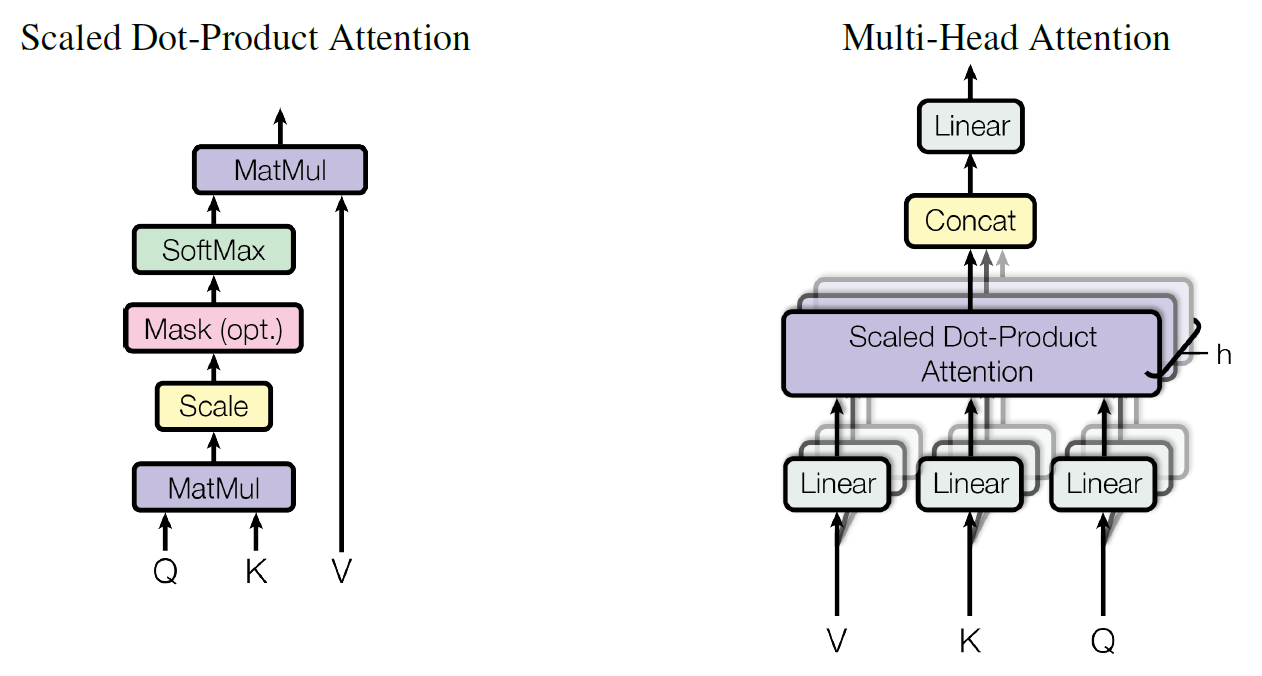
\includegraphics[width=\linewidth]{figure/scaled_multiheaded_attn.png}
    \caption{缩放后的多头注意力机制示意图\cite{attn17}}
    \label{attn}
\end{figure}

如图\ref{attn}所示,缩放后的多头注意力机制是Transformer模型的核心组件,它可以建模任意长度的序列中元素间的关系,允许每个元素在编码过程中访问与自己有关的上下文。这里仅介绍自注意力机制,用于解码的交叉注意力则不做介绍。$\bm{x}$为注意力力机制的输入,$\bm{z}$为输出,其前向传播过程可以表示为:
\begin{align}
    e_{ij}^{\left(h\right)}&=\frac{\left(\bm{W}_Q^{\left(h\right)}\bm{x}_i\right)^T\bm{W}_k^{\left(h\right)}\bm{x}_j}{\sqrt{d_z/H}} \label{attn-forward:1}\\
    \alpha_{ij}^{\left(h\right)}&=\frac{\exp{\left(e_{ij}^{\left(h\right)}\right)}}{\sum_{l=1}^{n}\exp{\left(e_{il}^{\left(h\right)}\right)}} \label{attn-forward:2}\\
    \bm{z}_i^{\left(h\right)}&=\sum_{j=1}^{n}{\alpha_{ij}^{\left(h\right)}\left(\bm{W}_V^{\left(h\right)}\bm{x}_j\right)}\\
    \bm{z}_i&=\mathrm{Concat}\left(\bm{z}_i^{\left(1\right)},\ldots,\bm{z}_i^{\left(H\right)}\right)  \label{attn-forward:4}
\end{align}

其中H为注意力头的数量,$\bm{W}$是可学习的权重,$\alpha_{ij}$又称作注意力权重,它编码了第$i$个元素到第$j$个元素的关系紧密程度,具有较强的可解释性。

\subsection{Transformer编码器}

\begin{figure}[]
    \centering
    \includegraphics[page=5]{figure/figures.pdf}
    \caption{Transformer编码器示意图\cite{attn17}}
    \label{trans-enc}
\end{figure}

如图\ref{trans-enc}所示,建立在自注意力机制之上,Transformer编码器交替使用了自注意力层和前馈网络层,并使用了归一化和残差连接。$\bm{y}$表示单层编码器的输出,与公式\ref{attn-forward:1}到\ref{attn-forward:4}一起,其前向传播过程可表示为:
\def\LN{\mathrm{LayerNorm}}
\begin{align}
{\widetilde{\bm{y}}}_i&=\LN\left(\bm{x}_i+\bm{z}_i\right)\\
\bm{y}_i&=\LN\left({\widetilde{\bm{y}}}_i+\bm{W}_2\left(ReLU\left(\bm{W}_1{\widetilde{\bm{y}}}_i\right)\right)\right.
\end{align}

其中$\bm{W}$可学习的是参数,$\LN$表示层归一化\cite{LayerN16}。$N$个这样的层叠加在一起组成了Transformer的编码器。可以发现,自注意力机制并不能捕获序列中元素的位置信息,而前馈网络层是对每个元素单独运算的,也不能捕获位置信息。因此,Transformer将输入序列中元素的位置信息进行嵌入,并叠加在了首层的输入上。

\section{其他神经网络构建单元}

\subsection{池化层}

池化层之前广泛应用于计算机视觉的网络中,一般用于降低空间维度的大小,以减小计算量,并提升特征的抽象程度。在自然语言处理相关模型中,池化层的使用比较灵活,比如对于自然语言句子中语义相关联的几个单词,或者整个句子,我们希望能得到它们一个全局的向量表示,就可以使用池化层来融合它们的表示。常用的池化层包括平均池化和最大池化。它们的前向传播过程非常简单。若需要池化的区域为R,则前向传播过程如下:
最大池化:
\begin{equation}
    y=\max_{i\in R}{x_i}
\end{equation}

平均池化:
\begin{equation}
    y=\frac{1}{\left|R\right|}\sum_{i\in R}x_i
\end{equation}

其反向传播算法较为特殊,值得特别进行讨论。池化层没有可学习的参数,它仅将梯度反向传播至它的输入层。对于最大池化,它将梯度传递给区域中最大的元素,即:
\begin{equation}
    \frac{\partial J}{\partial x_i}=\begin{cases}
        \frac{\partial J}{\partial y}, & x_i=\max_{j\in R}{x_j}\\
        0, & \mathrm{otherwise}
    \end{cases}
\end{equation}

平均池化则可以使用普通的求导方法,即:
\begin{equation}
    \frac{\partial J}{\partial x_i}=\frac{1}{\left|R\right|}\cdot\frac{\partial J}{\partial y}
\end{equation}

\subsection{嵌入层}

嵌入 (embedding) 层在自然语言相关的模型中非常常用。它能将现实中离散的概念转换成高维空间中的连续的向量。例如,它将自然语言中的每一个单词,或者将分类任务中的类别转换为它的向量表示。嵌入层与其他的神经网络模块不同,它的输入是离散的,这意味着,没有损失函数对输入的导数存在,它不能反向传播到更早的层中。所以嵌入层仅能作为神经网络的第一层。嵌入层的实现非常简单,类似于字典查找,即对于第n种概念,输出矩阵$\bm{W}$的第n行。也可看作是one-hot向量使用矩阵$\bm{W}$进行线性变换。$\bm{W}$是可学习的参数。对于反向传播,则是直接将输出的梯度传播到$\bm{W}$中被选中的行,其它行的梯度则为0。

\section{本章小结}

本章介绍对神经网络的运行原理:前向传播,反向传播,优化方法进行了介绍。并介绍了在自然语言相关任务中最常使用的神经网络模块:全连接前馈神经网络,循环神经网络和注意力神经网络,以及其他一些辅助模块。这些介绍也反应了神经网络在这一领域的发展历史。这些原理和模块也是后文构建方案的基础。
